% SOURCE: ../../edit-harness/results/frame_a/cells/cell_*_real_MIX_A_*.json
% !TEX encoding = UTF-8 Unicode
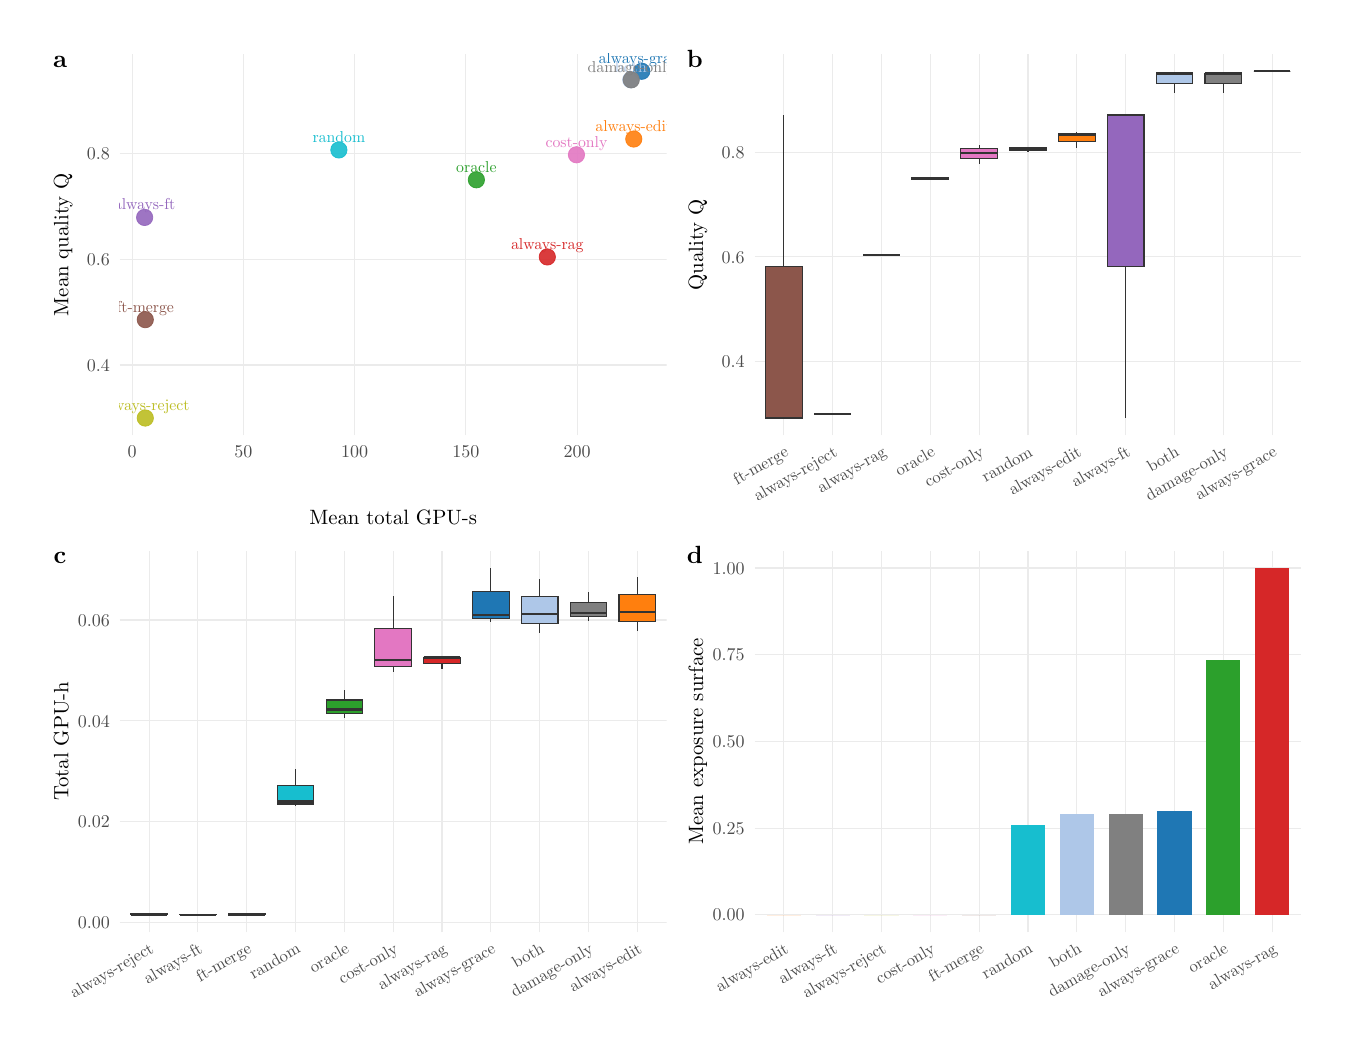
\begin{tikzpicture}[x=1pt,y=1pt]
\definecolor{fillColor}{RGB}{255,255,255}
\path[use as bounding box,fill=fillColor,fill opacity=0.00] (0,0) rectangle (469.75,361.35);
\begin{scope}
\path[clip] (  0.00,  0.00) rectangle (469.75,361.35);
\definecolor{drawColor}{RGB}{255,255,255}
\definecolor{fillColor}{RGB}{255,255,255}

\path[draw=drawColor,line width= 0.6pt,line join=round,line cap=round,fill=fillColor] (  0.00,  0.00) rectangle (469.75,361.35);
\end{scope}
\begin{scope}
\path[clip] (  5.50,176.36) rectangle (234.88,355.85);
\definecolor{fillColor}{RGB}{255,255,255}

\path[fill=fillColor] (  5.50,176.36) rectangle (234.88,355.85);
\end{scope}
\begin{scope}
\path[clip] (234.88,176.36) rectangle (464.25,355.85);
\definecolor{fillColor}{RGB}{255,255,255}

\path[fill=fillColor] (234.88,176.36) rectangle (464.25,355.85);
\end{scope}
\begin{scope}
\path[clip] (  5.50,  5.50) rectangle (234.88,176.36);
\definecolor{fillColor}{RGB}{255,255,255}

\path[fill=fillColor] (  5.50,  5.50) rectangle (234.88,176.36);
\end{scope}
\begin{scope}
\path[clip] (234.88,  5.50) rectangle (464.25,176.36);
\definecolor{fillColor}{RGB}{255,255,255}

\path[fill=fillColor] (234.88,  5.50) rectangle (464.25,176.36);
\end{scope}
\begin{scope}
\path[clip] ( 33.28,214.03) rectangle (230.88,351.85);
\definecolor{drawColor}{gray}{0.92}

\path[draw=drawColor,line width= 0.4pt,line join=round] ( 33.28,239.44) --
	(230.88,239.44);

\path[draw=drawColor,line width= 0.4pt,line join=round] ( 33.28,277.73) --
	(230.88,277.73);

\path[draw=drawColor,line width= 0.4pt,line join=round] ( 33.28,316.02) --
	(230.88,316.02);

\path[draw=drawColor,line width= 0.4pt,line join=round] ( 37.75,214.03) --
	( 37.75,351.85);

\path[draw=drawColor,line width= 0.4pt,line join=round] ( 77.96,214.03) --
	( 77.96,351.85);

\path[draw=drawColor,line width= 0.4pt,line join=round] (118.16,214.03) --
	(118.16,351.85);

\path[draw=drawColor,line width= 0.4pt,line join=round] (158.36,214.03) --
	(158.36,351.85);

\path[draw=drawColor,line width= 0.4pt,line join=round] (198.57,214.03) --
	(198.57,351.85);
\definecolor{drawColor}{RGB}{255,127,14}
\definecolor{fillColor}{RGB}{255,127,14}

\path[draw=drawColor,draw opacity=0.90,line width= 0.3pt,line join=round,line cap=round,fill=fillColor,fill opacity=0.90] (219.01,321.11) circle (  2.94);
\definecolor{drawColor}{RGB}{148,103,189}
\definecolor{fillColor}{RGB}{148,103,189}

\path[draw=drawColor,draw opacity=0.90,line width= 0.3pt,line join=round,line cap=round,fill=fillColor,fill opacity=0.90] ( 42.26,292.78) circle (  2.94);
\definecolor{drawColor}{RGB}{31,119,180}
\definecolor{fillColor}{RGB}{31,119,180}

\path[draw=drawColor,draw opacity=0.90,line width= 0.3pt,line join=round,line cap=round,fill=fillColor,fill opacity=0.90] (221.90,345.59) circle (  2.94);
\definecolor{drawColor}{RGB}{214,39,40}
\definecolor{fillColor}{RGB}{214,39,40}

\path[draw=drawColor,draw opacity=0.90,line width= 0.3pt,line join=round,line cap=round,fill=fillColor,fill opacity=0.90] (187.77,278.50) circle (  2.94);
\definecolor{drawColor}{RGB}{188,189,34}
\definecolor{fillColor}{RGB}{188,189,34}

\path[draw=drawColor,draw opacity=0.90,line width= 0.3pt,line join=round,line cap=round,fill=fillColor,fill opacity=0.90] ( 42.50,220.29) circle (  2.94);
\definecolor{drawColor}{RGB}{174,199,232}
\definecolor{fillColor}{RGB}{174,199,232}

\path[draw=drawColor,draw opacity=0.90,line width= 0.3pt,line join=round,line cap=round,fill=fillColor,fill opacity=0.90] (217.93,342.50) circle (  2.94);
\definecolor{drawColor}{RGB}{227,119,194}
\definecolor{fillColor}{RGB}{227,119,194}

\path[draw=drawColor,draw opacity=0.90,line width= 0.3pt,line join=round,line cap=round,fill=fillColor,fill opacity=0.90] (198.30,315.42) circle (  2.94);
\definecolor{drawColor}{RGB}{127,127,127}
\definecolor{fillColor}{RGB}{127,127,127}

\path[draw=drawColor,draw opacity=0.90,line width= 0.3pt,line join=round,line cap=round,fill=fillColor,fill opacity=0.90] (218.10,342.50) circle (  2.94);
\definecolor{drawColor}{RGB}{140,86,75}
\definecolor{fillColor}{RGB}{140,86,75}

\path[draw=drawColor,draw opacity=0.90,line width= 0.3pt,line join=round,line cap=round,fill=fillColor,fill opacity=0.90] ( 42.50,255.84) circle (  2.94);
\definecolor{drawColor}{RGB}{44,160,44}
\definecolor{fillColor}{RGB}{44,160,44}

\path[draw=drawColor,draw opacity=0.90,line width= 0.3pt,line join=round,line cap=round,fill=fillColor,fill opacity=0.90] (162.14,306.37) circle (  2.94);
\definecolor{drawColor}{RGB}{23,190,207}
\definecolor{fillColor}{RGB}{23,190,207}

\path[draw=drawColor,draw opacity=0.90,line width= 0.3pt,line join=round,line cap=round,fill=fillColor,fill opacity=0.90] (112.45,317.16) circle (  2.94);
\definecolor{drawColor}{RGB}{255,127,14}

\node[text=drawColor,anchor=base,inner sep=0pt, outer sep=0pt, scale=  0.57] at (219.01,323.86) {always-edit};
\definecolor{drawColor}{RGB}{148,103,189}

\node[text=drawColor,anchor=base,inner sep=0pt, outer sep=0pt, scale=  0.57] at ( 42.26,295.52) {always-ft};
\definecolor{drawColor}{RGB}{31,119,180}

\node[text=drawColor,anchor=base,inner sep=0pt, outer sep=0pt, scale=  0.57] at (221.90,348.33) {always-grace};
\definecolor{drawColor}{RGB}{214,39,40}

\node[text=drawColor,anchor=base,inner sep=0pt, outer sep=0pt, scale=  0.57] at (187.77,281.24) {always-rag};
\definecolor{drawColor}{RGB}{188,189,34}

\node[text=drawColor,anchor=base,inner sep=0pt, outer sep=0pt, scale=  0.57] at ( 42.50,223.04) {always-reject};
\definecolor{drawColor}{RGB}{174,199,232}

\node[text=drawColor,anchor=base,inner sep=0pt, outer sep=0pt, scale=  0.57] at (217.93,345.24) {both};
\definecolor{drawColor}{RGB}{227,119,194}

\node[text=drawColor,anchor=base,inner sep=0pt, outer sep=0pt, scale=  0.57] at (198.30,318.17) {cost-only};
\definecolor{drawColor}{gray}{0.50}

\node[text=drawColor,anchor=base,inner sep=0pt, outer sep=0pt, scale=  0.57] at (218.10,345.24) {damage-only};
\definecolor{drawColor}{RGB}{140,86,75}

\node[text=drawColor,anchor=base,inner sep=0pt, outer sep=0pt, scale=  0.57] at ( 42.50,258.58) {ft-merge};
\definecolor{drawColor}{RGB}{44,160,44}

\node[text=drawColor,anchor=base,inner sep=0pt, outer sep=0pt, scale=  0.57] at (162.14,309.12) {oracle};
\definecolor{drawColor}{RGB}{23,190,207}

\node[text=drawColor,anchor=base,inner sep=0pt, outer sep=0pt, scale=  0.57] at (112.45,319.90) {random};
\end{scope}
\begin{scope}
\path[clip] (  0.00,  0.00) rectangle (469.75,361.35);
\definecolor{drawColor}{gray}{0.30}

\node[text=drawColor,anchor=base east,inner sep=0pt, outer sep=0pt, scale=  0.65] at ( 29.68,237.20) {0.4};

\node[text=drawColor,anchor=base east,inner sep=0pt, outer sep=0pt, scale=  0.65] at ( 29.68,275.49) {0.6};

\node[text=drawColor,anchor=base east,inner sep=0pt, outer sep=0pt, scale=  0.65] at ( 29.68,313.79) {0.8};
\end{scope}
\begin{scope}
\path[clip] (  0.00,  0.00) rectangle (469.75,361.35);
\definecolor{drawColor}{gray}{0.30}

\node[text=drawColor,anchor=base,inner sep=0pt, outer sep=0pt, scale=  0.65] at ( 37.75,205.95) {0};

\node[text=drawColor,anchor=base,inner sep=0pt, outer sep=0pt, scale=  0.65] at ( 77.96,205.95) {50};

\node[text=drawColor,anchor=base,inner sep=0pt, outer sep=0pt, scale=  0.65] at (118.16,205.95) {100};

\node[text=drawColor,anchor=base,inner sep=0pt, outer sep=0pt, scale=  0.65] at (158.36,205.95) {150};

\node[text=drawColor,anchor=base,inner sep=0pt, outer sep=0pt, scale=  0.65] at (198.57,205.95) {200};
\end{scope}
\begin{scope}
\path[clip] (  0.00,  0.00) rectangle (469.75,361.35);
\definecolor{drawColor}{RGB}{0,0,0}

\node[text=drawColor,anchor=base,inner sep=0pt, outer sep=0pt, scale=  0.75] at (132.08,181.82) {Mean total GPU-s};
\end{scope}
\begin{scope}
\path[clip] (  0.00,  0.00) rectangle (469.75,361.35);
\definecolor{drawColor}{RGB}{0,0,0}

\node[text=drawColor,rotate= 90.00,anchor=base,inner sep=0pt, outer sep=0pt, scale=  0.75] at ( 14.67,282.94) {Mean quality Q};
\end{scope}
\begin{scope}
\path[clip] (  0.00,  0.00) rectangle (469.75,361.35);
\definecolor{drawColor}{RGB}{0,0,0}

\node[text=drawColor,anchor=base,inner sep=0pt, outer sep=0pt, scale=  0.90] at ( 11.71,347.03) {\bfseries a};
\end{scope}
\begin{scope}
\path[clip] (262.65,214.03) rectangle (460.25,351.85);
\definecolor{drawColor}{gray}{0.92}

\path[draw=drawColor,line width= 0.4pt,line join=round] (262.65,240.64) --
	(460.25,240.64);

\path[draw=drawColor,line width= 0.4pt,line join=round] (262.65,278.50) --
	(460.25,278.50);

\path[draw=drawColor,line width= 0.4pt,line join=round] (262.65,316.36) --
	(460.25,316.36);

\path[draw=drawColor,line width= 0.4pt,line join=round] (273.24,214.03) --
	(273.24,351.85);

\path[draw=drawColor,line width= 0.4pt,line join=round] (290.88,214.03) --
	(290.88,351.85);

\path[draw=drawColor,line width= 0.4pt,line join=round] (308.53,214.03) --
	(308.53,351.85);

\path[draw=drawColor,line width= 0.4pt,line join=round] (326.17,214.03) --
	(326.17,351.85);

\path[draw=drawColor,line width= 0.4pt,line join=round] (343.81,214.03) --
	(343.81,351.85);

\path[draw=drawColor,line width= 0.4pt,line join=round] (361.45,214.03) --
	(361.45,351.85);

\path[draw=drawColor,line width= 0.4pt,line join=round] (379.10,214.03) --
	(379.10,351.85);

\path[draw=drawColor,line width= 0.4pt,line join=round] (396.74,214.03) --
	(396.74,351.85);

\path[draw=drawColor,line width= 0.4pt,line join=round] (414.38,214.03) --
	(414.38,351.85);

\path[draw=drawColor,line width= 0.4pt,line join=round] (432.03,214.03) --
	(432.03,351.85);

\path[draw=drawColor,line width= 0.4pt,line join=round] (449.67,214.03) --
	(449.67,351.85);
\definecolor{drawColor}{gray}{0.20}

\path[draw=drawColor,line width= 0.4pt,line join=round] (273.24,275.13) -- (273.24,329.91);

\path[draw=drawColor,line width= 0.4pt,line join=round] (273.24,220.32) -- (273.24,220.29);
\definecolor{fillColor}{RGB}{140,86,75}

\path[draw=drawColor,line width= 0.4pt,fill=fillColor] (266.62,275.13) --
	(266.62,220.32) --
	(279.86,220.32) --
	(279.86,275.13) --
	(266.62,275.13) --
	cycle;

\path[draw=drawColor,line width= 0.8pt] (266.62,220.34) -- (279.86,220.34);

\path[draw=drawColor,line width= 0.4pt,line join=round] (290.88,221.71) -- (290.88,221.71);

\path[draw=drawColor,line width= 0.4pt,line join=round] (290.88,221.71) -- (290.88,221.71);
\definecolor{fillColor}{RGB}{188,189,34}

\path[draw=drawColor,line width= 0.4pt,fill=fillColor] (284.27,221.71) --
	(284.27,221.71) --
	(297.50,221.71) --
	(297.50,221.71) --
	(284.27,221.71) --
	cycle;

\path[draw=drawColor,line width= 0.8pt] (284.27,221.71) -- (297.50,221.71);

\path[draw=drawColor,line width= 0.4pt,line join=round] (308.53,279.26) -- (308.53,279.26);

\path[draw=drawColor,line width= 0.4pt,line join=round] (308.53,279.26) -- (308.53,279.26);
\definecolor{fillColor}{RGB}{214,39,40}

\path[draw=drawColor,line width= 0.4pt,fill=fillColor] (301.91,279.26) --
	(301.91,279.26) --
	(315.14,279.26) --
	(315.14,279.26) --
	(301.91,279.26) --
	cycle;

\path[draw=drawColor,line width= 0.8pt] (301.91,279.26) -- (315.14,279.26);

\path[draw=drawColor,line width= 0.4pt,line join=round] (326.17,307.04) -- (326.17,307.27);

\path[draw=drawColor,line width= 0.4pt,line join=round] (326.17,306.59) -- (326.17,306.36);
\definecolor{fillColor}{RGB}{44,160,44}

\path[draw=drawColor,line width= 0.4pt,fill=fillColor] (319.55,307.04) --
	(319.55,306.59) --
	(332.78,306.59) --
	(332.78,307.04) --
	(319.55,307.04) --
	cycle;

\path[draw=drawColor,line width= 0.8pt] (319.55,306.82) -- (332.78,306.82);

\path[draw=drawColor,line width= 0.4pt,line join=round] (343.81,317.66) -- (343.81,319.12);

\path[draw=drawColor,line width= 0.4pt,line join=round] (343.81,314.09) -- (343.81,311.97);
\definecolor{fillColor}{RGB}{227,119,194}

\path[draw=drawColor,line width= 0.4pt,fill=fillColor] (337.20,317.66) --
	(337.20,314.09) --
	(350.43,314.09) --
	(350.43,317.66) --
	(337.20,317.66) --
	cycle;

\path[draw=drawColor,line width= 0.8pt] (337.20,316.20) -- (350.43,316.20);

\path[draw=drawColor,line width= 0.4pt,line join=round] (361.45,318.06) -- (361.45,318.18);

\path[draw=drawColor,line width= 0.4pt,line join=round] (361.45,317.13) -- (361.45,316.32);
\definecolor{fillColor}{RGB}{23,190,207}

\path[draw=drawColor,line width= 0.4pt,fill=fillColor] (354.84,318.06) --
	(354.84,317.13) --
	(368.07,317.13) --
	(368.07,318.06) --
	(354.84,318.06) --
	cycle;

\path[draw=drawColor,line width= 0.8pt] (354.84,317.93) -- (368.07,317.93);

\path[draw=drawColor,line width= 0.4pt,line join=round] (379.10,323.22) -- (379.10,323.82);

\path[draw=drawColor,line width= 0.4pt,line join=round] (379.10,320.17) -- (379.10,317.73);
\definecolor{fillColor}{RGB}{255,127,14}

\path[draw=drawColor,line width= 0.4pt,fill=fillColor] (372.48,323.22) --
	(372.48,320.17) --
	(385.71,320.17) --
	(385.71,323.22) --
	(372.48,323.22) --
	cycle;

\path[draw=drawColor,line width= 0.8pt] (372.48,322.61) -- (385.71,322.61);

\path[draw=drawColor,line width= 0.4pt,line join=round] (396.74,329.91) -- (396.74,329.91);

\path[draw=drawColor,line width= 0.4pt,line join=round] (396.74,275.10) -- (396.74,220.29);
\definecolor{fillColor}{RGB}{148,103,189}

\path[draw=drawColor,line width= 0.4pt,fill=fillColor] (390.12,329.91) --
	(390.12,275.10) --
	(403.36,275.10) --
	(403.36,329.91) --
	(390.12,329.91) --
	cycle;

\path[draw=drawColor,line width= 0.8pt] (390.12,329.91) -- (403.36,329.91);

\path[draw=drawColor,line width= 0.4pt,line join=round] (414.38,344.89) -- (414.38,345.00);

\path[draw=drawColor,line width= 0.4pt,line join=round] (414.38,341.30) -- (414.38,337.82);
\definecolor{fillColor}{RGB}{174,199,232}

\path[draw=drawColor,line width= 0.4pt,fill=fillColor] (407.77,344.89) --
	(407.77,341.30) --
	(421.00,341.30) --
	(421.00,344.89) --
	(407.77,344.89) --
	cycle;

\path[draw=drawColor,line width= 0.8pt] (407.77,344.78) -- (421.00,344.78);

\path[draw=drawColor,line width= 0.4pt,line join=round] (432.03,344.89) -- (432.03,345.00);

\path[draw=drawColor,line width= 0.4pt,line join=round] (432.03,341.30) -- (432.03,337.82);
\definecolor{fillColor}{gray}{0.50}

\path[draw=drawColor,line width= 0.4pt,fill=fillColor] (425.41,344.89) --
	(425.41,341.30) --
	(438.64,341.30) --
	(438.64,344.89) --
	(425.41,344.89) --
	cycle;

\path[draw=drawColor,line width= 0.8pt] (425.41,344.78) -- (438.64,344.78);

\path[draw=drawColor,line width= 0.4pt,line join=round] (449.67,345.59) -- (449.67,345.59);

\path[draw=drawColor,line width= 0.4pt,line join=round] (449.67,345.59) -- (449.67,345.59);
\definecolor{fillColor}{RGB}{31,119,180}

\path[draw=drawColor,line width= 0.4pt,fill=fillColor] (443.05,345.59) --
	(443.05,345.59) --
	(456.29,345.59) --
	(456.29,345.59) --
	(443.05,345.59) --
	cycle;

\path[draw=drawColor,line width= 0.8pt] (443.05,345.59) -- (456.29,345.59);
\end{scope}
\begin{scope}
\path[clip] (  0.00,  0.00) rectangle (469.75,361.35);
\definecolor{drawColor}{gray}{0.30}

\node[text=drawColor,anchor=base east,inner sep=0pt, outer sep=0pt, scale=  0.65] at (259.05,238.40) {0.4};

\node[text=drawColor,anchor=base east,inner sep=0pt, outer sep=0pt, scale=  0.65] at (259.05,276.26) {0.6};

\node[text=drawColor,anchor=base east,inner sep=0pt, outer sep=0pt, scale=  0.65] at (259.05,314.12) {0.8};
\end{scope}
\begin{scope}
\path[clip] (  0.00,  0.00) rectangle (469.75,361.35);
\definecolor{drawColor}{gray}{0.30}

\node[text=drawColor,rotate= 30.00,anchor=base east,inner sep=0pt, outer sep=0pt, scale=  0.60] at (275.31,206.85) {ft-merge};

\node[text=drawColor,rotate= 30.00,anchor=base east,inner sep=0pt, outer sep=0pt, scale=  0.60] at (292.95,206.85) {always-reject};

\node[text=drawColor,rotate= 30.00,anchor=base east,inner sep=0pt, outer sep=0pt, scale=  0.60] at (310.59,206.85) {always-rag};

\node[text=drawColor,rotate= 30.00,anchor=base east,inner sep=0pt, outer sep=0pt, scale=  0.60] at (328.23,206.85) {oracle};

\node[text=drawColor,rotate= 30.00,anchor=base east,inner sep=0pt, outer sep=0pt, scale=  0.60] at (345.88,206.85) {cost-only};

\node[text=drawColor,rotate= 30.00,anchor=base east,inner sep=0pt, outer sep=0pt, scale=  0.60] at (363.52,206.85) {random};

\node[text=drawColor,rotate= 30.00,anchor=base east,inner sep=0pt, outer sep=0pt, scale=  0.60] at (381.16,206.85) {always-edit};

\node[text=drawColor,rotate= 30.00,anchor=base east,inner sep=0pt, outer sep=0pt, scale=  0.60] at (398.81,206.85) {always-ft};

\node[text=drawColor,rotate= 30.00,anchor=base east,inner sep=0pt, outer sep=0pt, scale=  0.60] at (416.45,206.85) {both};

\node[text=drawColor,rotate= 30.00,anchor=base east,inner sep=0pt, outer sep=0pt, scale=  0.60] at (434.09,206.85) {damage-only};

\node[text=drawColor,rotate= 30.00,anchor=base east,inner sep=0pt, outer sep=0pt, scale=  0.60] at (451.74,206.85) {always-grace};
\end{scope}
\begin{scope}
\path[clip] (  0.00,  0.00) rectangle (469.75,361.35);
\definecolor{drawColor}{RGB}{0,0,0}

\node[text=drawColor,rotate= 90.00,anchor=base,inner sep=0pt, outer sep=0pt, scale=  0.75] at (244.04,282.94) {Quality Q};
\end{scope}
\begin{scope}
\path[clip] (  0.00,  0.00) rectangle (469.75,361.35);
\definecolor{drawColor}{RGB}{0,0,0}

\node[text=drawColor,anchor=base,inner sep=0pt, outer sep=0pt, scale=  0.90] at (241.09,347.03) {\bfseries b};
\end{scope}
\begin{scope}
\path[clip] ( 33.28, 34.54) rectangle (230.88,172.36);
\definecolor{drawColor}{gray}{0.92}

\path[draw=drawColor,line width= 0.4pt,line join=round] ( 33.28, 38.01) --
	(230.88, 38.01);

\path[draw=drawColor,line width= 0.4pt,line join=round] ( 33.28, 74.44) --
	(230.88, 74.44);

\path[draw=drawColor,line width= 0.4pt,line join=round] ( 33.28,110.87) --
	(230.88,110.87);

\path[draw=drawColor,line width= 0.4pt,line join=round] ( 33.28,147.30) --
	(230.88,147.30);

\path[draw=drawColor,line width= 0.4pt,line join=round] ( 43.86, 34.54) --
	( 43.86,172.36);

\path[draw=drawColor,line width= 0.4pt,line join=round] ( 61.50, 34.54) --
	( 61.50,172.36);

\path[draw=drawColor,line width= 0.4pt,line join=round] ( 79.15, 34.54) --
	( 79.15,172.36);

\path[draw=drawColor,line width= 0.4pt,line join=round] ( 96.79, 34.54) --
	( 96.79,172.36);

\path[draw=drawColor,line width= 0.4pt,line join=round] (114.43, 34.54) --
	(114.43,172.36);

\path[draw=drawColor,line width= 0.4pt,line join=round] (132.08, 34.54) --
	(132.08,172.36);

\path[draw=drawColor,line width= 0.4pt,line join=round] (149.72, 34.54) --
	(149.72,172.36);

\path[draw=drawColor,line width= 0.4pt,line join=round] (167.36, 34.54) --
	(167.36,172.36);

\path[draw=drawColor,line width= 0.4pt,line join=round] (185.01, 34.54) --
	(185.01,172.36);

\path[draw=drawColor,line width= 0.4pt,line join=round] (202.65, 34.54) --
	(202.65,172.36);

\path[draw=drawColor,line width= 0.4pt,line join=round] (220.29, 34.54) --
	(220.29,172.36);
\definecolor{drawColor}{gray}{0.20}

\path[draw=drawColor,line width= 0.4pt,line join=round] ( 43.86, 41.09) -- ( 43.86, 41.35);

\path[draw=drawColor,line width= 0.4pt,line join=round] ( 43.86, 40.82) -- ( 43.86, 40.81);
\definecolor{fillColor}{RGB}{188,189,34}

\path[draw=drawColor,line width= 0.4pt,fill=fillColor] ( 37.25, 41.09) --
	( 37.25, 40.82) --
	( 50.48, 40.82) --
	( 50.48, 41.09) --
	( 37.25, 41.09) --
	cycle;

\path[draw=drawColor,line width= 0.8pt] ( 37.25, 40.82) -- ( 50.48, 40.82);

\path[draw=drawColor,line width= 0.4pt,line join=round] ( 61.50, 40.86) -- ( 61.50, 40.90);

\path[draw=drawColor,line width= 0.4pt,line join=round] ( 61.50, 40.82) -- ( 61.50, 40.81);
\definecolor{fillColor}{RGB}{148,103,189}

\path[draw=drawColor,line width= 0.4pt,fill=fillColor] ( 54.89, 40.86) --
	( 54.89, 40.82) --
	( 68.12, 40.82) --
	( 68.12, 40.86) --
	( 54.89, 40.86) --
	cycle;

\path[draw=drawColor,line width= 0.8pt] ( 54.89, 40.82) -- ( 68.12, 40.82);

\path[draw=drawColor,line width= 0.4pt,line join=round] ( 79.15, 41.09) -- ( 79.15, 41.31);

\path[draw=drawColor,line width= 0.4pt,line join=round] ( 79.15, 40.84) -- ( 79.15, 40.81);
\definecolor{fillColor}{RGB}{140,86,75}

\path[draw=drawColor,line width= 0.4pt,fill=fillColor] ( 72.53, 41.09) --
	( 72.53, 40.84) --
	( 85.76, 40.84) --
	( 85.76, 41.09) --
	( 72.53, 41.09) --
	cycle;

\path[draw=drawColor,line width= 0.8pt] ( 72.53, 40.87) -- ( 85.76, 40.87);

\path[draw=drawColor,line width= 0.4pt,line join=round] ( 96.79, 87.55) -- ( 96.79, 93.36);

\path[draw=drawColor,line width= 0.4pt,line join=round] ( 96.79, 80.84) -- ( 96.79, 79.95);
\definecolor{fillColor}{RGB}{23,190,207}

\path[draw=drawColor,line width= 0.4pt,fill=fillColor] ( 90.17, 87.55) --
	( 90.17, 80.84) --
	(103.41, 80.84) --
	(103.41, 87.55) --
	( 90.17, 87.55) --
	cycle;

\path[draw=drawColor,line width= 0.8pt] ( 90.17, 81.73) -- (103.41, 81.73);

\path[draw=drawColor,line width= 0.4pt,line join=round] (114.43,118.41) -- (114.43,121.84);

\path[draw=drawColor,line width= 0.4pt,line join=round] (114.43,113.50) -- (114.43,112.03);
\definecolor{fillColor}{RGB}{44,160,44}

\path[draw=drawColor,line width= 0.4pt,fill=fillColor] (107.82,118.41) --
	(107.82,113.50) --
	(121.05,113.50) --
	(121.05,118.41) --
	(107.82,118.41) --
	cycle;

\path[draw=drawColor,line width= 0.8pt] (107.82,114.97) -- (121.05,114.97);

\path[draw=drawColor,line width= 0.4pt,line join=round] (132.08,144.39) -- (132.08,156.01);

\path[draw=drawColor,line width= 0.4pt,line join=round] (132.08,130.55) -- (132.08,128.34);
\definecolor{fillColor}{RGB}{227,119,194}

\path[draw=drawColor,line width= 0.4pt,fill=fillColor] (125.46,144.39) --
	(125.46,130.55) --
	(138.69,130.55) --
	(138.69,144.39) --
	(125.46,144.39) --
	cycle;

\path[draw=drawColor,line width= 0.8pt] (125.46,132.76) -- (138.69,132.76);

\path[draw=drawColor,line width= 0.4pt,line join=round] (149.72,133.85) -- (149.72,133.94);

\path[draw=drawColor,line width= 0.4pt,line join=round] (149.72,131.65) -- (149.72,129.54);
\definecolor{fillColor}{RGB}{214,39,40}

\path[draw=drawColor,line width= 0.4pt,fill=fillColor] (143.10,133.85) --
	(143.10,131.65) --
	(156.34,131.65) --
	(156.34,133.85) --
	(143.10,133.85) --
	cycle;

\path[draw=drawColor,line width= 0.8pt] (143.10,133.77) -- (156.34,133.77);

\path[draw=drawColor,line width= 0.4pt,line join=round] (167.36,157.56) -- (167.36,166.10);

\path[draw=drawColor,line width= 0.4pt,line join=round] (167.36,147.78) -- (167.36,146.55);
\definecolor{fillColor}{RGB}{31,119,180}

\path[draw=drawColor,line width= 0.4pt,fill=fillColor] (160.75,157.56) --
	(160.75,147.78) --
	(173.98,147.78) --
	(173.98,157.56) --
	(160.75,157.56) --
	cycle;

\path[draw=drawColor,line width= 0.8pt] (160.75,149.01) -- (173.98,149.01);

\path[draw=drawColor,line width= 0.4pt,line join=round] (185.01,155.84) -- (185.01,162.11);

\path[draw=drawColor,line width= 0.4pt,line join=round] (185.01,146.03) -- (185.01,142.49);
\definecolor{fillColor}{RGB}{174,199,232}

\path[draw=drawColor,line width= 0.4pt,fill=fillColor] (178.39,155.84) --
	(178.39,146.03) --
	(191.62,146.03) --
	(191.62,155.84) --
	(178.39,155.84) --
	cycle;

\path[draw=drawColor,line width= 0.8pt] (178.39,149.57) -- (191.62,149.57);

\path[draw=drawColor,line width= 0.4pt,line join=round] (202.65,153.70) -- (202.65,157.50);

\path[draw=drawColor,line width= 0.4pt,line join=round] (202.65,148.50) -- (202.65,147.09);
\definecolor{fillColor}{gray}{0.50}

\path[draw=drawColor,line width= 0.4pt,fill=fillColor] (196.03,153.70) --
	(196.03,148.50) --
	(209.26,148.50) --
	(209.26,153.70) --
	(196.03,153.70) --
	cycle;

\path[draw=drawColor,line width= 0.8pt] (196.03,149.91) -- (209.26,149.91);

\path[draw=drawColor,line width= 0.4pt,line join=round] (220.29,156.49) -- (220.29,162.72);

\path[draw=drawColor,line width= 0.4pt,line join=round] (220.29,146.75) -- (220.29,143.25);
\definecolor{fillColor}{RGB}{255,127,14}

\path[draw=drawColor,line width= 0.4pt,fill=fillColor] (213.68,156.49) --
	(213.68,146.75) --
	(226.91,146.75) --
	(226.91,156.49) --
	(213.68,156.49) --
	cycle;

\path[draw=drawColor,line width= 0.8pt] (213.68,150.25) -- (226.91,150.25);
\end{scope}
\begin{scope}
\path[clip] (  0.00,  0.00) rectangle (469.75,361.35);
\definecolor{drawColor}{gray}{0.30}

\node[text=drawColor,anchor=base east,inner sep=0pt, outer sep=0pt, scale=  0.65] at ( 29.68, 35.77) {0.00};

\node[text=drawColor,anchor=base east,inner sep=0pt, outer sep=0pt, scale=  0.65] at ( 29.68, 72.20) {0.02};

\node[text=drawColor,anchor=base east,inner sep=0pt, outer sep=0pt, scale=  0.65] at ( 29.68,108.63) {0.04};

\node[text=drawColor,anchor=base east,inner sep=0pt, outer sep=0pt, scale=  0.65] at ( 29.68,145.07) {0.06};
\end{scope}
\begin{scope}
\path[clip] (  0.00,  0.00) rectangle (469.75,361.35);
\definecolor{drawColor}{gray}{0.30}

\node[text=drawColor,rotate= 30.00,anchor=base east,inner sep=0pt, outer sep=0pt, scale=  0.60] at ( 45.93, 27.36) {always-reject};

\node[text=drawColor,rotate= 30.00,anchor=base east,inner sep=0pt, outer sep=0pt, scale=  0.60] at ( 63.57, 27.36) {always-ft};

\node[text=drawColor,rotate= 30.00,anchor=base east,inner sep=0pt, outer sep=0pt, scale=  0.60] at ( 81.21, 27.36) {ft-merge};

\node[text=drawColor,rotate= 30.00,anchor=base east,inner sep=0pt, outer sep=0pt, scale=  0.60] at ( 98.86, 27.36) {random};

\node[text=drawColor,rotate= 30.00,anchor=base east,inner sep=0pt, outer sep=0pt, scale=  0.60] at (116.50, 27.36) {oracle};

\node[text=drawColor,rotate= 30.00,anchor=base east,inner sep=0pt, outer sep=0pt, scale=  0.60] at (134.14, 27.36) {cost-only};

\node[text=drawColor,rotate= 30.00,anchor=base east,inner sep=0pt, outer sep=0pt, scale=  0.60] at (151.79, 27.36) {always-rag};

\node[text=drawColor,rotate= 30.00,anchor=base east,inner sep=0pt, outer sep=0pt, scale=  0.60] at (169.43, 27.36) {always-grace};

\node[text=drawColor,rotate= 30.00,anchor=base east,inner sep=0pt, outer sep=0pt, scale=  0.60] at (187.07, 27.36) {both};

\node[text=drawColor,rotate= 30.00,anchor=base east,inner sep=0pt, outer sep=0pt, scale=  0.60] at (204.71, 27.36) {damage-only};

\node[text=drawColor,rotate= 30.00,anchor=base east,inner sep=0pt, outer sep=0pt, scale=  0.60] at (222.36, 27.36) {always-edit};
\end{scope}
\begin{scope}
\path[clip] (  0.00,  0.00) rectangle (469.75,361.35);
\definecolor{drawColor}{RGB}{0,0,0}

\node[text=drawColor,rotate= 90.00,anchor=base,inner sep=0pt, outer sep=0pt, scale=  0.75] at ( 14.67,103.45) {Total GPU-h};
\end{scope}
\begin{scope}
\path[clip] (  0.00,  0.00) rectangle (469.75,361.35);
\definecolor{drawColor}{RGB}{0,0,0}

\node[text=drawColor,anchor=base,inner sep=0pt, outer sep=0pt, scale=  0.90] at ( 11.71,167.63) {\bfseries c};
\end{scope}
\begin{scope}
\path[clip] (262.65, 34.54) rectangle (460.25,172.36);
\definecolor{drawColor}{gray}{0.92}

\path[draw=drawColor,line width= 0.4pt,line join=round] (262.65, 40.81) --
	(460.25, 40.81);

\path[draw=drawColor,line width= 0.4pt,line join=round] (262.65, 72.13) --
	(460.25, 72.13);

\path[draw=drawColor,line width= 0.4pt,line join=round] (262.65,103.45) --
	(460.25,103.45);

\path[draw=drawColor,line width= 0.4pt,line join=round] (262.65,134.78) --
	(460.25,134.78);

\path[draw=drawColor,line width= 0.4pt,line join=round] (262.65,166.10) --
	(460.25,166.10);

\path[draw=drawColor,line width= 0.4pt,line join=round] (273.24, 34.54) --
	(273.24,172.36);

\path[draw=drawColor,line width= 0.4pt,line join=round] (290.88, 34.54) --
	(290.88,172.36);

\path[draw=drawColor,line width= 0.4pt,line join=round] (308.53, 34.54) --
	(308.53,172.36);

\path[draw=drawColor,line width= 0.4pt,line join=round] (326.17, 34.54) --
	(326.17,172.36);

\path[draw=drawColor,line width= 0.4pt,line join=round] (343.81, 34.54) --
	(343.81,172.36);

\path[draw=drawColor,line width= 0.4pt,line join=round] (361.45, 34.54) --
	(361.45,172.36);

\path[draw=drawColor,line width= 0.4pt,line join=round] (379.10, 34.54) --
	(379.10,172.36);

\path[draw=drawColor,line width= 0.4pt,line join=round] (396.74, 34.54) --
	(396.74,172.36);

\path[draw=drawColor,line width= 0.4pt,line join=round] (414.38, 34.54) --
	(414.38,172.36);

\path[draw=drawColor,line width= 0.4pt,line join=round] (432.03, 34.54) --
	(432.03,172.36);

\path[draw=drawColor,line width= 0.4pt,line join=round] (449.67, 34.54) --
	(449.67,172.36);
\definecolor{fillColor}{RGB}{255,127,14}

\path[fill=fillColor] (267.06, 40.81) rectangle (279.41, 40.81);
\definecolor{fillColor}{RGB}{148,103,189}

\path[fill=fillColor] (284.71, 40.81) rectangle (297.06, 40.81);
\definecolor{fillColor}{RGB}{31,119,180}

\path[fill=fillColor] (408.21, 40.81) rectangle (420.56, 78.40);
\definecolor{fillColor}{RGB}{214,39,40}

\path[fill=fillColor] (443.49, 40.81) rectangle (455.84,166.10);
\definecolor{fillColor}{RGB}{188,189,34}

\path[fill=fillColor] (302.35, 40.81) rectangle (314.70, 40.81);
\definecolor{fillColor}{RGB}{174,199,232}

\path[fill=fillColor] (372.92, 40.81) rectangle (385.27, 77.34);
\definecolor{fillColor}{RGB}{227,119,194}

\path[fill=fillColor] (319.99, 40.81) rectangle (332.34, 40.81);
\definecolor{fillColor}{gray}{0.50}

\path[fill=fillColor] (390.57, 40.81) rectangle (402.92, 77.34);
\definecolor{fillColor}{RGB}{140,86,75}

\path[fill=fillColor] (337.64, 40.81) rectangle (349.99, 40.81);
\definecolor{fillColor}{RGB}{44,160,44}

\path[fill=fillColor] (425.85, 40.81) rectangle (438.20,132.71);
\definecolor{fillColor}{RGB}{23,190,207}

\path[fill=fillColor] (355.28, 40.81) rectangle (367.63, 73.09);
\end{scope}
\begin{scope}
\path[clip] (  0.00,  0.00) rectangle (469.75,361.35);
\definecolor{drawColor}{gray}{0.30}

\node[text=drawColor,anchor=base east,inner sep=0pt, outer sep=0pt, scale=  0.65] at (259.05, 38.57) {0.00};

\node[text=drawColor,anchor=base east,inner sep=0pt, outer sep=0pt, scale=  0.65] at (259.05, 69.89) {0.25};

\node[text=drawColor,anchor=base east,inner sep=0pt, outer sep=0pt, scale=  0.65] at (259.05,101.21) {0.50};

\node[text=drawColor,anchor=base east,inner sep=0pt, outer sep=0pt, scale=  0.65] at (259.05,132.54) {0.75};

\node[text=drawColor,anchor=base east,inner sep=0pt, outer sep=0pt, scale=  0.65] at (259.05,163.86) {1.00};
\end{scope}
\begin{scope}
\path[clip] (  0.00,  0.00) rectangle (469.75,361.35);
\definecolor{drawColor}{gray}{0.30}

\node[text=drawColor,rotate= 30.00,anchor=base east,inner sep=0pt, outer sep=0pt, scale=  0.60] at (275.31, 27.36) {always-edit};

\node[text=drawColor,rotate= 30.00,anchor=base east,inner sep=0pt, outer sep=0pt, scale=  0.60] at (292.95, 27.36) {always-ft};

\node[text=drawColor,rotate= 30.00,anchor=base east,inner sep=0pt, outer sep=0pt, scale=  0.60] at (310.59, 27.36) {always-reject};

\node[text=drawColor,rotate= 30.00,anchor=base east,inner sep=0pt, outer sep=0pt, scale=  0.60] at (328.23, 27.36) {cost-only};

\node[text=drawColor,rotate= 30.00,anchor=base east,inner sep=0pt, outer sep=0pt, scale=  0.60] at (345.88, 27.36) {ft-merge};

\node[text=drawColor,rotate= 30.00,anchor=base east,inner sep=0pt, outer sep=0pt, scale=  0.60] at (363.52, 27.36) {random};

\node[text=drawColor,rotate= 30.00,anchor=base east,inner sep=0pt, outer sep=0pt, scale=  0.60] at (381.16, 27.36) {both};

\node[text=drawColor,rotate= 30.00,anchor=base east,inner sep=0pt, outer sep=0pt, scale=  0.60] at (398.81, 27.36) {damage-only};

\node[text=drawColor,rotate= 30.00,anchor=base east,inner sep=0pt, outer sep=0pt, scale=  0.60] at (416.45, 27.36) {always-grace};

\node[text=drawColor,rotate= 30.00,anchor=base east,inner sep=0pt, outer sep=0pt, scale=  0.60] at (434.09, 27.36) {oracle};

\node[text=drawColor,rotate= 30.00,anchor=base east,inner sep=0pt, outer sep=0pt, scale=  0.60] at (451.74, 27.36) {always-rag};
\end{scope}
\begin{scope}
\path[clip] (  0.00,  0.00) rectangle (469.75,361.35);
\definecolor{drawColor}{RGB}{0,0,0}

\node[text=drawColor,rotate= 90.00,anchor=base,inner sep=0pt, outer sep=0pt, scale=  0.75] at (244.04,103.45) {Mean exposure surface};
\end{scope}
\begin{scope}
\path[clip] (  0.00,  0.00) rectangle (469.75,361.35);
\definecolor{drawColor}{RGB}{0,0,0}

\node[text=drawColor,anchor=base,inner sep=0pt, outer sep=0pt, scale=  0.90] at (241.09,167.63) {\bfseries d};
\end{scope}
\end{tikzpicture}
